
%% overclocking_tcad.tex
%% by Kan Shi


%\usepackage{times,epsfig,amsfonts,bm}
%\usepackage{pdflscape}
%\usepackage{afterpage}
%\usepackage{algorithm}
%\usepackage{algorithmic}
%\usepackage{fmtcount,threeparttable, setspace, nicefrac}
%\usepackage[dvips]{color}
%\usepackage{amsthm}

\documentclass[journal]{IEEEtran}
\usepackage{cite}

\ifCLASSINFOpdf
  \usepackage[pdftex]{graphicx}
  % declare the path(s) where your graphic files are
  % \graphicspath{{../pdf/}{../jpeg/}}
  % and their extensions so you won't have to specify these with
  % every instance of \includegraphics
  % \DeclareGraphicsExtensions{.pdf,.jpeg,.png}
\else
  % or other class option (dvipsone, dvipdf, if not using dvips). graphicx
  % will default to the driver specified in the system graphics.cfg if no
  % driver is specified.
  \usepackage[dvips]{graphicx}
  % declare the path(s) where your graphic files are
  \graphicspath{{../Figures/}}
  % and their extensions so you won't have to specify these with
  % every instance of \includegraphics
  \DeclareGraphicsExtensions{.eps}
\fi
\usepackage{epstopdf}


\usepackage{multirow}
\usepackage{amssymb}
\usepackage[cmex10]{amsmath}
%\usepackage{algorithmic}
%\usepackage{array}
\usepackage[tight,footnotesize]{subfigure}
\usepackage{stfloats}



\begin{document}

\title{Title}

\author{Kan~Shi,
        David~Boland,~\IEEEmembership{Member,~IEEE,}
        and~George~A.~Constantinides,~\IEEEmembership{Senior~Member,~IEEE}% <-this % stops a space
	\thanks{K. Shi, D. Boland and G. A. Constantinides are with the Department of Electrical and Electronic Engineering, Imperial College London, London, SW7 2BT, U.K. (email: {}@imperial.ac.uk)}%
	%\thanks{M. Shell is with the Department of Electrical and Computer Engineering, Georgia Institute of Technology, Atlanta,GA, 30332 USA e-mail: (see http://www.michaelshell.org/contact.html).}% <-this % stops a space
%\thanks{J. Doe and J. Doe are with Anonymous University.}% <-this % stops a space
\thanks{Manuscript received April 19, 2005; revised December 27, 2012.}}

% note the % following the last \IEEEmembership and also \thanks - 
% these prevent an unwanted space from occurring between the last author name
% and the end of the author line. i.e., if you had this:
% 
% \author{....lastname \thanks{...} \thanks{...} }
%                     ^------------^------------^----Do not want these spaces!
%
% a space would be appended to the last name and could cause every name on that
% line to be shifted left slightly. This is one of those "LaTeX things". For
% instance, "\textbf{A} \textbf{B}" will typeset as "A B" not "AB". To get
% "AB" then you have to do: "\textbf{A}\textbf{B}"
% \thanks is no different in this regard, so shield the last } of each \thanks
% that ends a line with a % and do not let a space in before the next \thanks.
% Spaces after \IEEEmembership other than the last one are OK (and needed) as
% you are supposed to have spaces between the names. For what it is worth,
% this is a minor point as most people would not even notice if the said evil
% space somehow managed to creep in.



% The paper headers
\markboth{Journal of \LaTeX\ Class Files,~Vol.~11, No.~4, December~2012}%
{Shell \MakeLowercase{\textit{et al.}}: Bare Demo of IEEEtran.cls for Journals}

\maketitle

% As a general rule, do not put math, special symbols or citations
% in the abstract or keywords.
\begin{abstract}
The abstract.
\end{abstract}

\begin{IEEEkeywords}

\end{IEEEkeywords}


% For peer review papers, you can put extra information on the cover
% page as needed:
% \ifCLASSOPTIONpeerreview
% \begin{center} \bfseries EDICS Category: 3-BBND \end{center}
% \fi
%
% For peerreview papers, this IEEEtran command inserts a page break and
% creates the second title. It will be ignored for other modes.
\IEEEpeerreviewmaketitle



\section{Introduction}
% The very first letter is a 2 line initial drop letter followed
% by the rest of the first word in caps.
% 
% form to use if the first word consists of a single letter:
% \IEEEPARstart{A}{demo} file is ....
% 
% form to use if you need the single drop letter followed by
% normal text (unknown if ever used by IEEE):
% \IEEEPARstart{A}{}demo file is ....
% 
% Some journals put the first two words in caps:
% \IEEEPARstart{T}{his demo} file is ....
% 
% Here we have the typical use of a "T" for an initial drop letter
% and "HIS" in caps to complete the first word.
\IEEEPARstart{T}{his} demo file is intended to serve as a ``starter file''
for IEEE journal papers produced under \LaTeX\ using
IEEEtran.cls version 1.8 and later.
% You must have at least 2 lines in the paragraph with the drop letter
% (should never be an issue)
I wish you the best of success.

\hfill mds
 
\hfill December 27, 2012

\subsection{Subsection Heading Here}
Subsection text here.


\subsubsection{Subsubsection Heading Here}
Subsubsection text here.

\section{Carry Select Adder}
\subsection{Introduction}
Since the delay of RCA is determined by the length of carry chain, there are several alternative adder architectures proposed to shorten the carry chain. For instance, the carry select adder (CSA) is designed to overlap carry propagation in sections such that the operating speed can be boosted. In a CSA, the carry chain is divided into multiple stages. Each stage contains two RCAs and two multiplexers. For a given input, computations are performed twice simultaneously, with the carry input as zero and one respectively. The results are then selected according to the actual carry input. Although this structure brings timing benefits, it costs extra hardware resources than RCA as the carry chain is duplicated and multiplexers are expensive especially in the FPGA technology. In this section, silicon area is incorporated as the third metric besides accuracy and performance. We explore the trade-offs between these three factors for both adder structures. The objective is to demonstrate the best design choice for a given set of design constraints.

%In addition to RCA, there are several 

\subsection{Timing Models for $n$-bit Carry Select Adder}
We initially describe the modelling method for the CSA timing, with the aim of forming the relationship between the operating frequency and the corresponding maximum word-length of CSA. This information can be employed to determine the truncation error based on the models presented in Section.xxx.

In a CSA with $c$ stages, let the stage delay be denoted by $d_{0}\dots d_{c-1}$, where $d_{0}$ and $d_{c-1}$ represent the delay of the most significant stage and the least significant stage, respectively. Unlike other stages, the least significant stage is built by one RCA only, since it is directly driven by the carry input. In our analysis, we follow the previous assumption that delay is due to carry propagation as well as, in this case, multiplexing the carry output. Therefore the delay of the $i^{th}$ stage can be obtained through~(\ref{CSA_SingleStageDelay}), where $\mu_{c}$ denotes the delay of $1$-bit carry propagation and $\mu_{mux}$ denotes the delay of multiplexing.
\begin{eqnarray}\label{CSA_SingleStageDelay}
  d_i=n_i\cdot \mu_{c}+(i+1)\cdot\mu_{mux} 
 % d_0=n_0\cdot \mu_{carry}+\mu_{mux}
\end{eqnarray}

Under the timing-driven design environment, the delay of each stage of CSA is set to be approximately uniform for the fastest operation. In this case we obtain~(\ref{CSA_DelayEqual}).
\begin{eqnarray}\label{CSA_DelayEqual}
  d_0=d_1=\cdots=d_{n-1}
\end{eqnarray}

Substituting (\ref{CSA_SingleStageDelay}) into (\ref{CSA_DelayEqual}) yields (\ref{CSA_DelayRep}), which denotes the CSA word-length of stage $i$. Note that the word-length of stage $c-1$ and $c-2$ are identical, since the least significant stage is composed of RCA.
\begin{eqnarray}\label{CSA_DelayRep}
 % n_i=n_0-xxx\cdot\frac{\mu_{mux}}{\mu_{c}}
 n_i=\left\{
	\begin{matrix}
	  n_0-i\cdot\frac{\mu_{mux}}{\mu_c}, & \textrm{if $i\in(2,c-2]$ and $c>2$}\\
	  n_0-(c-2)\cdot\frac{\mu_{mux}}{\mu_c}, & \textrm{if $i=c-1$ and $c\geqslant2$}
	\end{matrix}
    \right.
\end{eqnarray}

The word-length of CSA is then given by (\ref{CSA_WL}).
\begin{eqnarray}\label{CSA_WL}
  n_{CSA}=\sum_{i=0}^{n-1}n_{i}=cn_{0}-\frac{\mu_{mux}}{\mu_{carry}}\cdot\frac{(c+1)(c-2)}{2}
\end{eqnarray}

In the conventional situation, the word-length of both RCA and CSA should be properly selected in order to meet timing. In this case,~(\ref{CSA_RCA}) can be obtained, where $n_{RCA}$ is determined by current timing information through (xxx).
\begin{eqnarray}\label{CSA_RCA}
  \mu_{c}\cdot n_{RCA}=\mu_{c}n_0+\mu_{mux}
\end{eqnarray}

Based on~(\ref{CSA_WL}) and~(\ref{CSA_RCA}), we may obtain the representation of the word-length of CSA in terms of a given timing constraint, as presented in~(\ref{CSA_Timing}).
% we form the relationship between the word-length of CSA and RCA under a given timing constraint, as presented in~(\ref{CSA_Timing}).
\begin{eqnarray}\label{CSA_Timing}
  n_{CSA}=c\cdot n_{RCA}-\frac{\mu_{mux}}{\mu_{c}}\cdot\frac{(c+2)(c-1)}{2}
\end{eqnarray}

It can be seen that $c=1$ leads to $n_{CSA}=n_{RCA}$. This is because RCA forms the least significant stage of CSA. In addition, combine (\ref{CSA_DelayRep}) and (\ref{CSA_RCA}) to ensure $n_{c-1}>0$, we obtain the upper bond of the stage number by~(\ref{CSA_StageNumber}).
\begin{eqnarray}\label{CSA_StageNumber}
  c<n_{RCA}\cdot\frac{\mu_c}{\mu_{mux}}+1
\end{eqnarray}
%the word-length of each CSA stage is allocated to ensure that 

\subsection{Model Verification}
As seen in (\ref{CSA_Timing}), the value of $\mu_{mux}/\mu_c$ should be determined before applying the timing model. This ratio can be obtained through timing analysis. Specifically, varying the word-length of a single stage $n_i$ and recording the corresponding delay value $d_i$ through the timing analysis tool. According to~(\ref{CSA_SingleStageDelay}), the ratio can be obtained by fitting those values using linear polynomials, as presented in Fig.~(\ref{DelayFitting}). Out experimental results show that $\mu_{mux}/\mu_c\approx8$.
%keeping $i=0$ in (\ref{CSA_SingleStageDelay}) while varying the value of $n_0$. The corresponding delay value $d_0$ is recorded through the timing analysis tool. Hence $\mu_{mux}/\mu_c$ can be obtained by fitting those values, as presented in Fig.~(\ref{DelayFitting}). Out experimental results show that $\mu_{mux}/\mu_c\approx8$.
\begin{figure}[htbp]
  \centering
  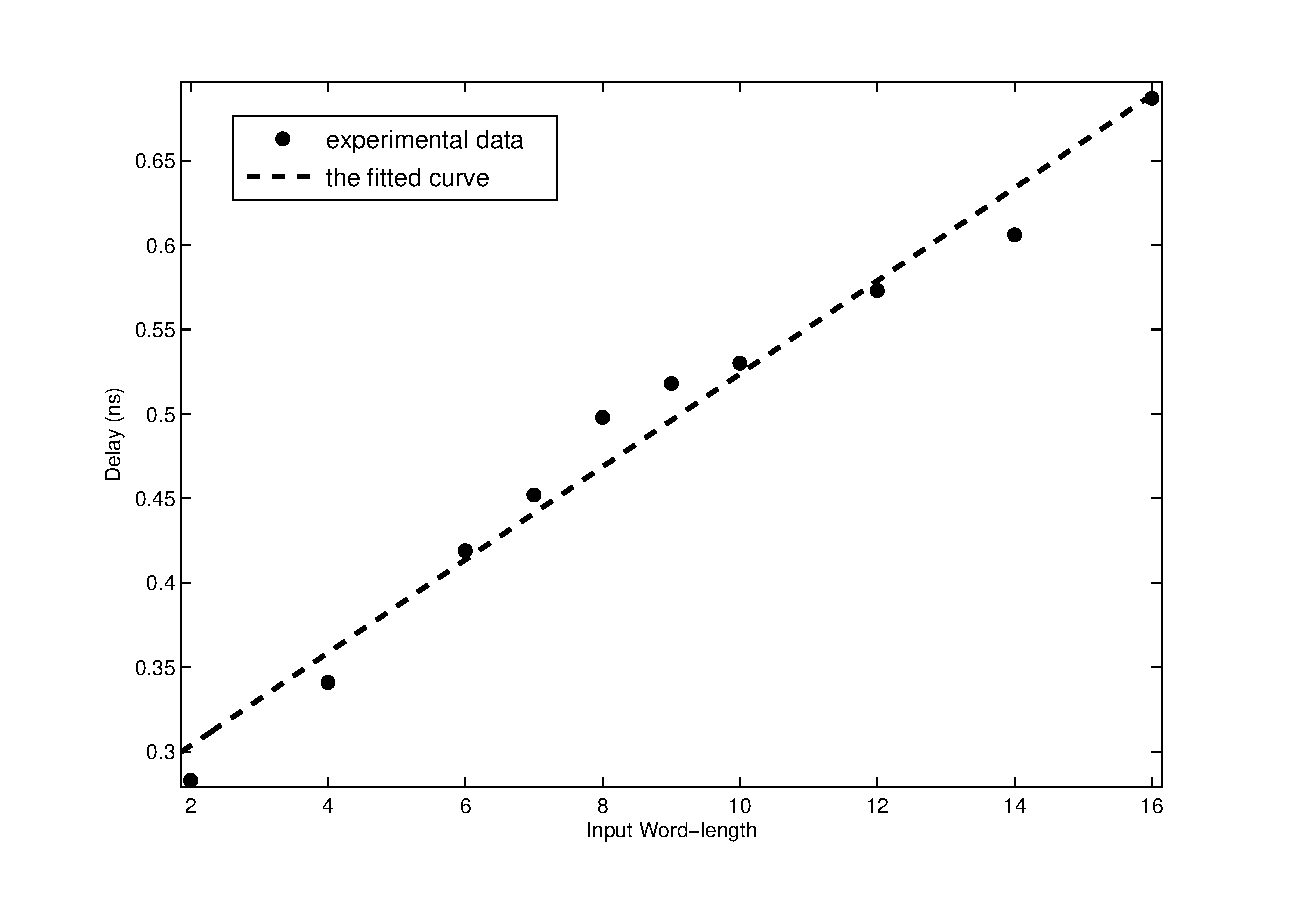
\includegraphics[width=3.3in]{./Figures/Fitting.eps}
  \caption{Fitted curve of (\ref{CSA_SingleStageDelay}) for the most significant stage ($i=0$), based on the given input word-length and the corresponding delay value obtained through the Xilinx Timing Analyzer.}
  \label{DelayFitting}
\end{figure}

Using this information, we verify our timing model with experimental results, which are obtained from post place and route simulations on Xilinx Virtex-6 FPGAs. Fig.~\ref{CSA Model Verification} demonstrates both the modelled value and the experimental results of the maximum word-length of RCA and 2-stage CSA, respectively, across a range of operating frequencies. The maximum input word-length in our experiments is 16-bit, hence the modelled value is set to 16 if it expires. 
\begin{figure}[htbp]
  \centering
  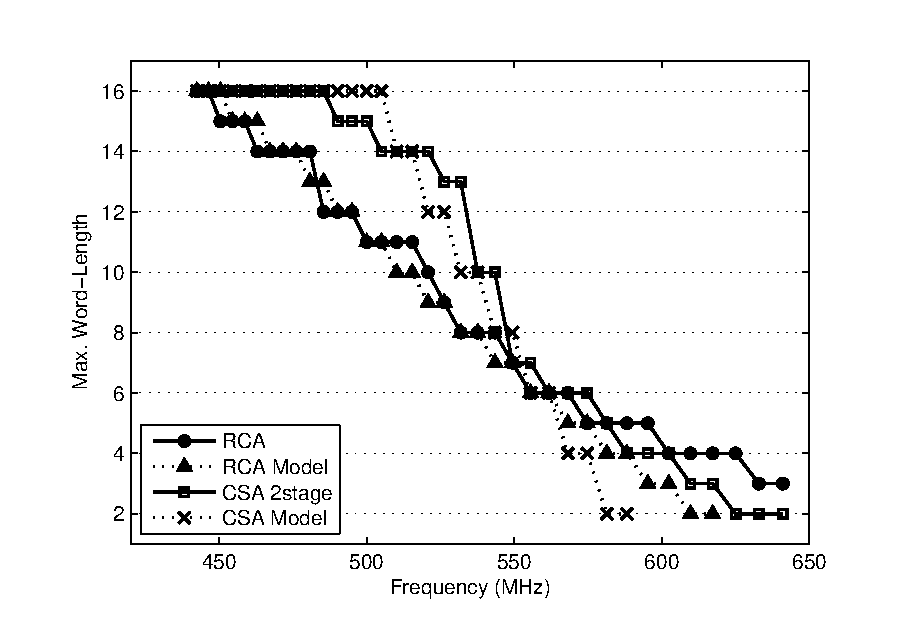
\includegraphics[width=3in]{./Figures/Model.eps}
  \caption{Comparison of the maximum word-length for a given operating frequency between the modelled value and the experimental results from FPGA simulations.}
  \label{CSA Model Verification}
\end{figure}

% Figure goes here!
It can be seen that our timing models match well the experimental results for both RCA and CSA, except that the modelled outcomes are slight conservative, especially at higher operating frequencies. This is because the model coefficients are obtained based on timing analysis, which is designed with safety margins to ensure correct functionality for diverse operating conditions. In addition, routing delay might be introduced during timing analysis such that the overall delay is enlarged, while our models consider logic delay only.

% provide slight conservative outcomes than the experimental data, especially at higher operating frequencies. 
. 

\subsection{Area Overhead}
Fig.~\ref{CSA3stage Timing} demonstrates the maximum word-lengths for RCA and CSA with 2 stages and 3 stages under a range of operating frequencies. We only investigate 3 stages as the maximum stages number predicted in (\ref{CSA_StageNumber}) is 3. It can be seen that in comparison to RCA, CSA achieves greater word-length when frequency is initially increased. This corresponds to smaller truncation errors. RCA only outperforms than CSA when very high frequency is applied. In addition, the word-length of 3-stage CSA is always greater than 2-stage CSA across the entire frequency domain, as expected.  
\begin{figure}[htbp]
  \centering
  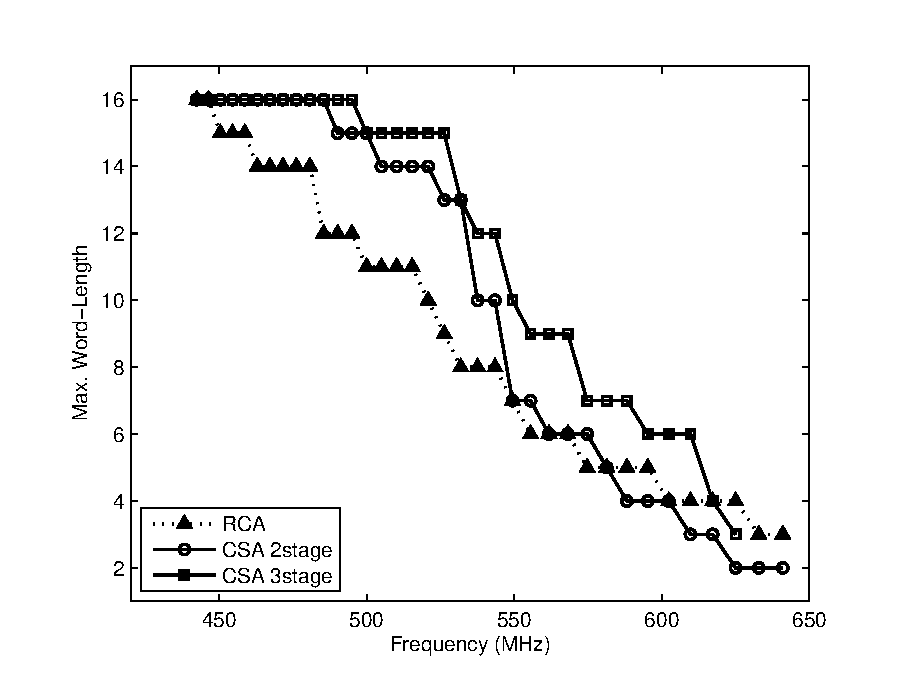
\includegraphics[width=3.3in]{./Figures/CSA3stage_Timing.eps}
  \caption{Maximum word-length for RCA and CSA across a variety of frequencies.}
  \label{CSA3stage Timing}
\end{figure}
%CSA achieves greater word-length than RCA when frequency is initially increased

However, the accuracy benefits brought by CSA comes with the cost of large area overhead. Fig.~\ref{CSA3stage Area} depicts the resource usage (in terms of the number of Look-Up Tables (LUTs) in the FPGA) used for all three structures. It can be seen that for a given frequency, the 3-stage CSA consumes $2.4\times\sim3.7\times$ area than RCA, while the number of the 2-stage CSA is $1.7\times\sim3.1\times$. This finding poses a question of whether CSA with higher stage numbers still offer better accuracy than RCA under a limited area budget.
\begin{figure}[htbp]
  \centering
  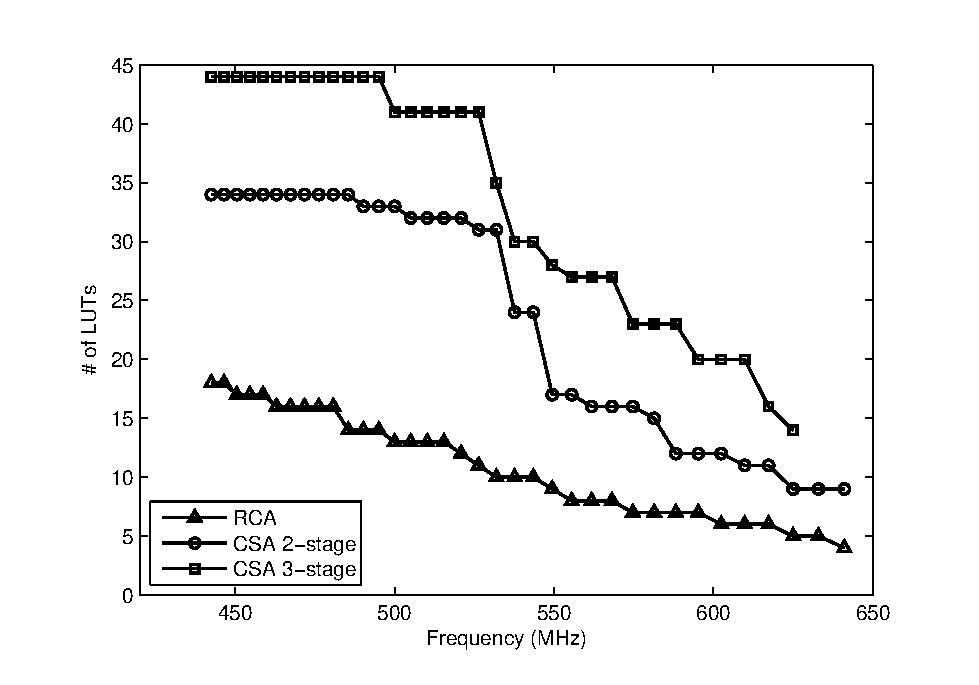
\includegraphics[width=3.3in]{./Figures/CSA3stage_Area.eps}
  \caption{Area overhead for RCA and CSA.}
  \label{CSA3stage Area}
\end{figure}
%the 3-stage CSA costs 

\subsection{Exploring Trade-offs Between Accuracy, Performance and Area}
%Although advanced architectures such as CSA inheritly offer better performance than the basic structure, this would generate a large area overhead. In the following experiments, 
To answer this question, we explore the trade-offs between accuracy, performance as well as area in this section. If the available hardware resources are limited, the full word-length of both CSA and RCA might not be implemented. The precision lose might generates large errors even at low frequencies. This is demonstrated by experiments where an area constraint is applied besides the timing requirement. Both of the constraints are met by reducing the word-length of the input signal. The errors at the outputs are recorded with the reference to the original word-length. In addition, another designing method is adopted where RCA is implemented with the maximum possible word-length under the given area budget, while the timing constraints are met by overclocking. For instance, Fig.xxx to Fig.xxx illustrate error expectations of all the described design scenarios when setting the LUTs number to 45, 35, 25 and 15 respectively. The optimal design metric with the minimum error expectation is labelled for each area constraint.
%
% the number of available LUTs is set to 45, 35, 25 and 15 respectively, while timing requirements are met by reducing the input word-length of each architecture. In addition, we also investigate the scenario where RCA is implemented with the maximum possible word-length under the given area constraint, while meeting timing by overclocking. The corresponding error expectations of these scenarios are depicted in Fig.xxx. The optimal design method which achieves the minimum error expectation is labelled.
\begin{figure}[htbp]
	\centering
	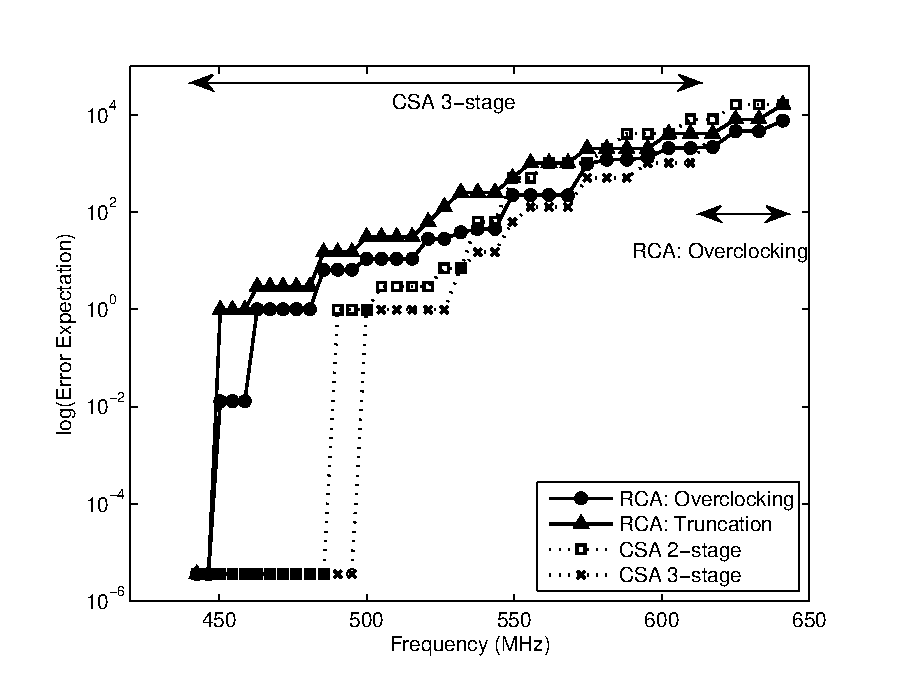
\includegraphics[width=3.3in]{./Figures/Error_LUT45.eps}
	\caption{LUT=45}
\end{figure}

\begin{figure}[htbp]
	\centering
	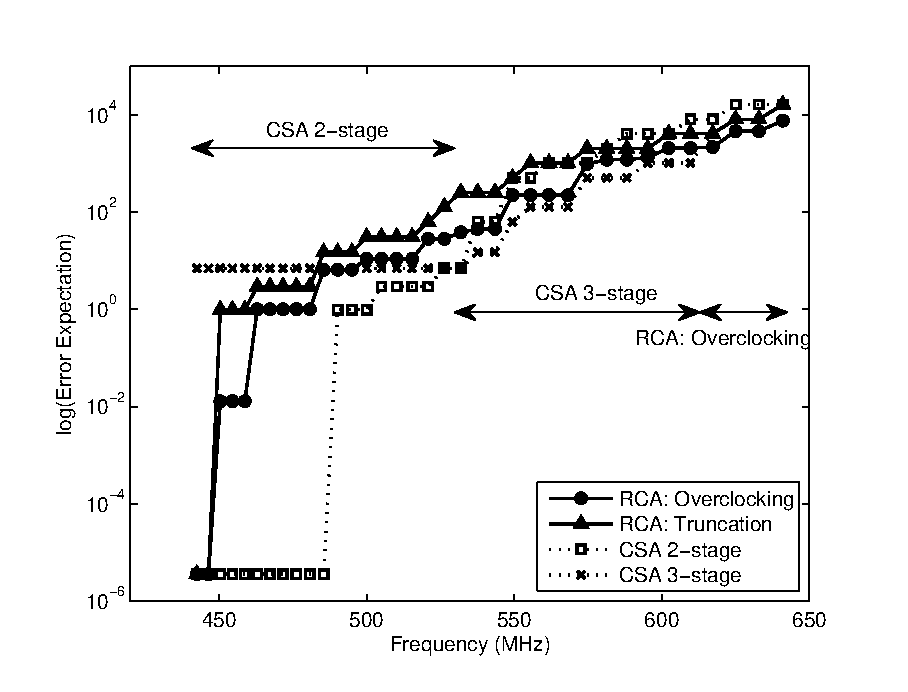
\includegraphics[width=3.3in]{./Figures/Error_LUT35.eps}
	\caption{LUT=35}
\end{figure}

\begin{figure}[htbp]
	\centering
	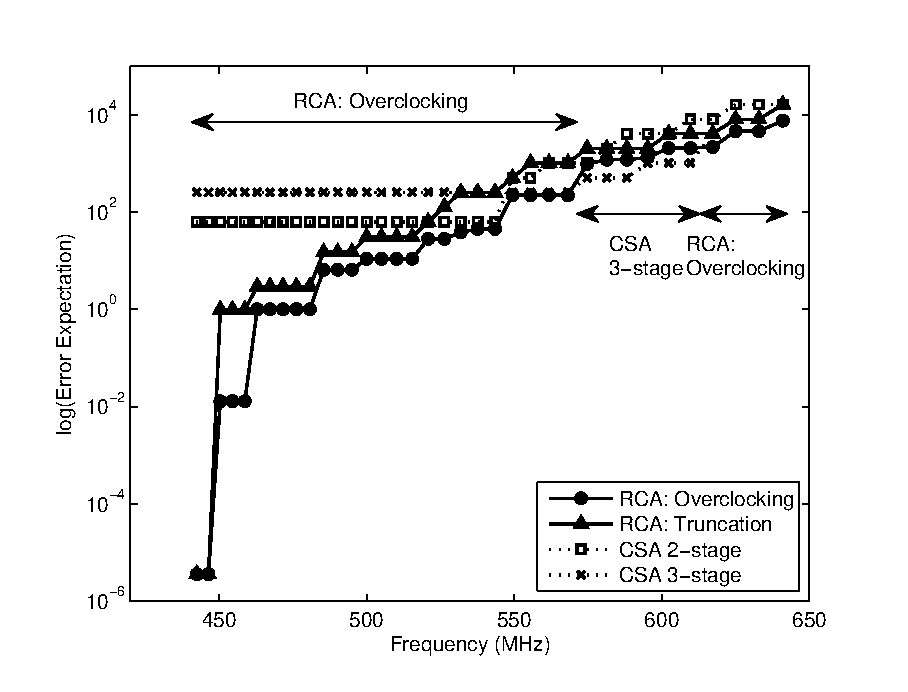
\includegraphics[width=3.3in]{./Figures/Error_LUT25.eps}
	\caption{LUT=25}
\end{figure}

\begin{figure}[htbp]
	\centering
	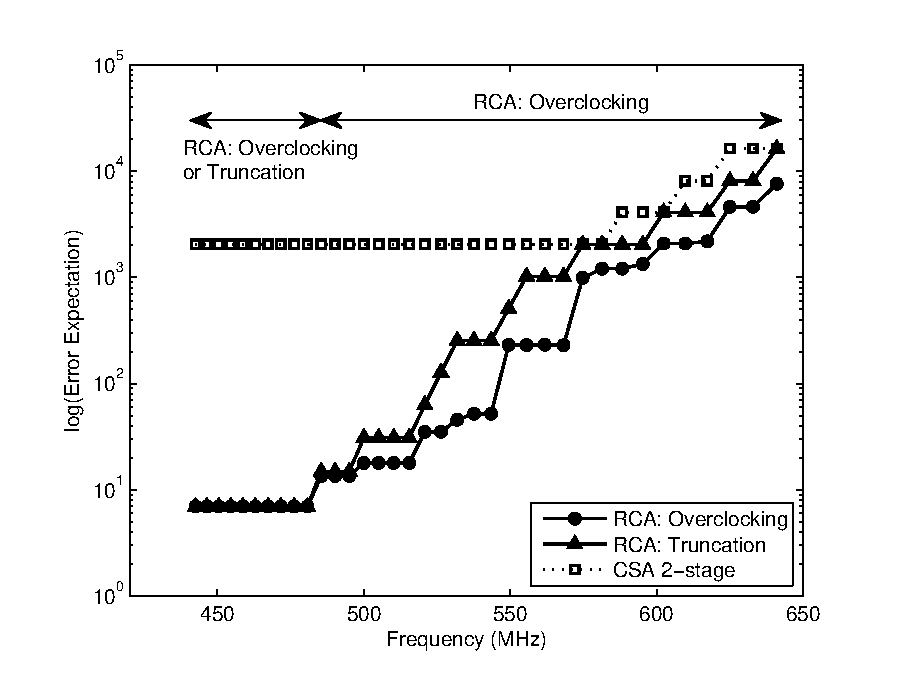
\includegraphics[width=3.3in]{./Figures/Error_LUT15.eps}
	\caption{LUT=15}
\end{figure}

%\begin{figure*}[htbp]
%  \centering
%  \subfigure[LUTs=45]{
%  \begin{minipage}[c]{0.45\textwidth}
%    \centering
%    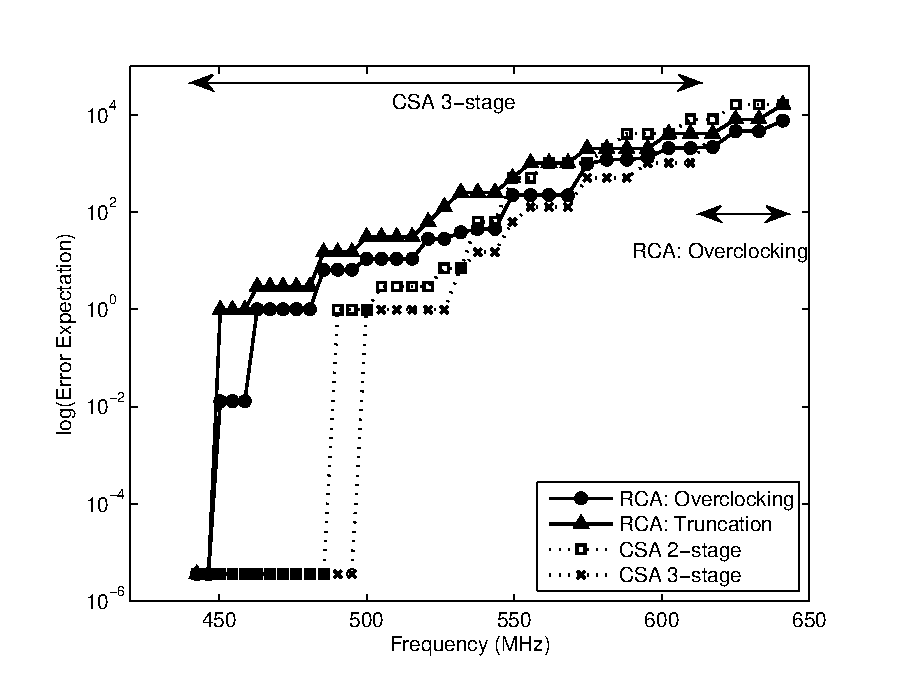
\includegraphics[width=2in]{./Figures/Error_LUT45.eps}
%  \end{minipage}%
%  }%
%  \subfigure[LUT=35]{
%  \begin{minipage}[c]{0.45\textwidth}
%    \centering
%    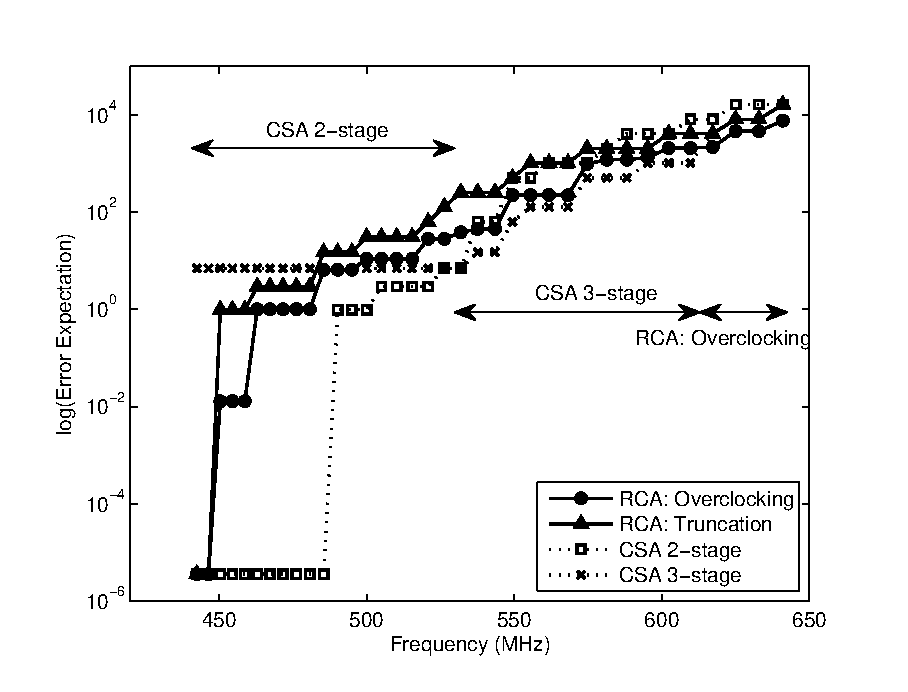
\includegraphics[width=2in]{./Figures/Error_LUT35.eps}
%  \end{minipage}
%  }
%  \subfigure[LUT=25]{
%  \begin{minipage}[c]{0.45\textwidth}
%    \centering
%    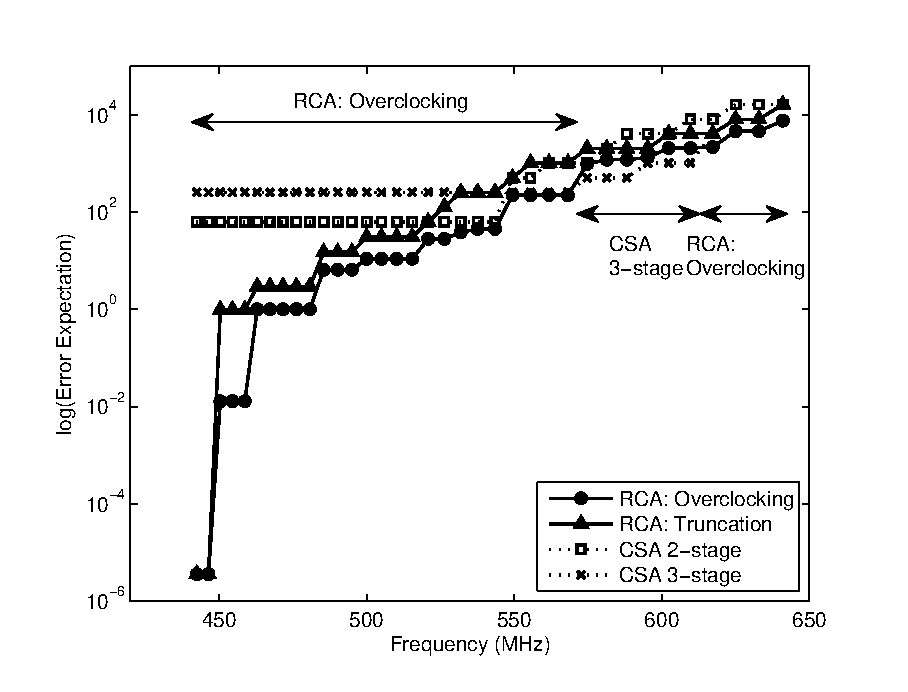
\includegraphics[width=2in]{./Figures/Error_LUT25.eps}
%  \end{minipage}
%  }%
%  \subfigure[LUT=15]{
%  \begin{minipage}[c]{0.45\textwidth}
%    \centering
%    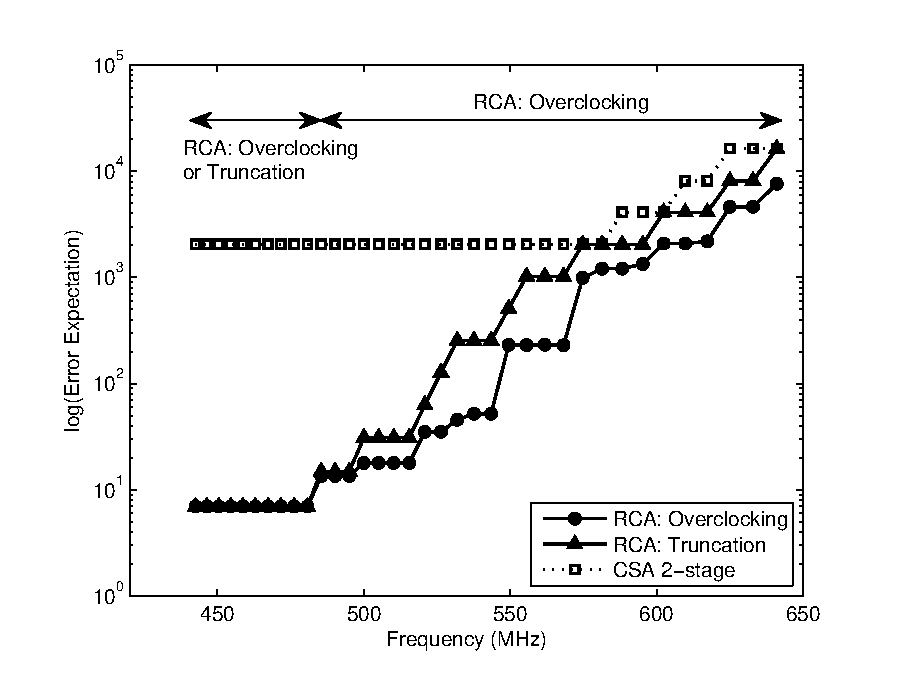
\includegraphics[width=2in]{./Figures/Error_LUT15.eps}
%  \end{minipage}
%  }
%  \caption{Accuracy-performance trade-offs under fixed area constraints.}
%  \label{Fig Tradeoffs}
%\end{figure*}

If the available area is large enough, as shown in Fig.xxx, CSA with higher stage numbers can be implemented with full precision and it is the optimal design choice unless very high frequencies are applied. This is because at lower frequencies, the long carry chain is divided into multiple overlapped sections, and the higher stage number the shorter the carry chain length of each stage. When the frequency increases, however, the multiplexer delay becomes comparable to the carry chain delay, and this will limit the maximum word-length of CSA. It can be seen that the overclocked RCA achieves best accuracy at higher frequencies.

For a tighter area budget, only part of the complex structures can be implemented, whilst the simple structure still keeps full precision. As can be seen in Fig.xxx and Fig.xxx, area instead of timing becomes the dominate factor when frequency is initially increased. This lead to a large truncation error for both 2-stage and 3-stage CSA. In this situation, overclocking RCA serves as the optimum choice with respect to accuracy.

For an even stringent area constraint, the word-length of RCA is also limited. This results in truncation error initially for all design scenarios, as shown in Fig.xxx. Meanwhile, CSA with high stage numbers could not be implemented at all. In this situation the overclocked RCA achieves best accuracy across the whole frequency domain.

In general, the error expectations at the output of all four design method for a set of timing and area constraints are demonstrated in Fig.~\ref{Tradeoff}.
\begin{figure}[htbp]
  \centering
  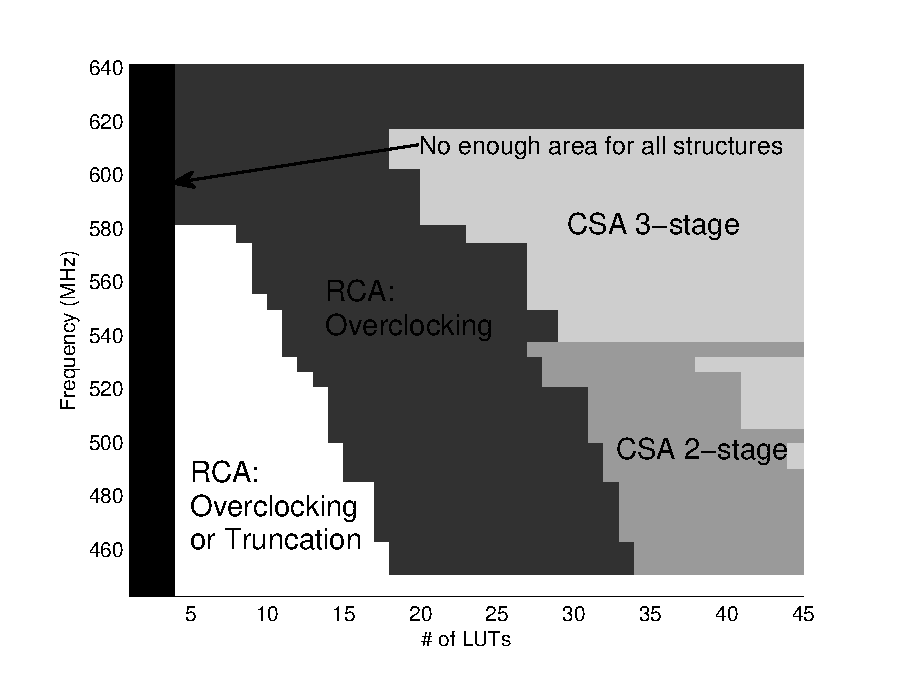
\includegraphics[width=3.3in]{./Figures/Tradeoff.eps}
  \caption{Trade-offs between accuracy, performance and area for 4 design methodologies.}
  \label{Tradeoff}
\end{figure}


% An example of a floating figure using the graphicx package.
% Note that \label must occur AFTER (or within) \caption.
% For figures, \caption should occur after the \includegraphics.
% Note that IEEEtran v1.7 and later has special internal code that
% is designed to preserve the operation of \label within \caption
% even when the captionsoff option is in effect. However, because
% of issues like this, it may be the safest practice to put all your
% \label just after \caption rather than within \caption{}.
%
% Reminder: the "draftcls" or "draftclsnofoot", not "draft", class
% option should be used if it is desired that the figures are to be
% displayed while in draft mode.
%
%\begin{figure}[!t]
%\centering
%\includegraphics[width=2.5in]{myfigure}
% where an .eps filename suffix will be assumed under latex, 
% and a .pdf suffix will be assumed for pdflatex; or what has been declared
% via \DeclareGraphicsExtensions.
%\caption{Simulation Results.}
%\label{fig_sim}
%\end{figure}

% Note that IEEE typically puts floats only at the top, even when this
% results in a large percentage of a column being occupied by floats.


% An example of a double column floating figure using two subfigures.
% (The subfig.sty package must be loaded for this to work.)
% The subfigure \label commands are set within each subfloat command,
% and the \label for the overall figure must come after \caption.
% \hfil is used as a separator to get equal spacing.
% Watch out that the combined width of all the subfigures on a 
% line do not exceed the text width or a line break will occur.
%
%\begin{figure*}[!t]
%\centering
%\subfloat[Case I]{\includegraphics[width=2.5in]{box}%
%\label{fig_first_case}}
%\hfil
%\subfloat[Case II]{\includegraphics[width=2.5in]{box}%
%\label{fig_second_case}}
%\caption{Simulation results.}
%\label{fig_sim}
%\end{figure*}
%
% Note that often IEEE papers with subfigures do not employ subfigure
% captions (using the optional argument to \subfloat[]), but instead will
% reference/describe all of them (a), (b), etc., within the main caption.


% An example of a floating table. Note that, for IEEE style tables, the 
% \caption command should come BEFORE the table. Table text will default to
% \footnotesize as IEEE normally uses this smaller font for tables.
% The \label must come after \caption as always.
%
%\begin{table}[!t]
%% increase table row spacing, adjust to taste
%\renewcommand{\arraystretch}{1.3}
% if using array.sty, it might be a good idea to tweak the value of
% \extrarowheight as needed to properly center the text within the cells
%\caption{An Example of a Table}
%\label{table_example}
%\centering
%% Some packages, such as MDW tools, offer better commands for making tables
%% than the plain LaTeX2e tabular which is used here.
%\begin{tabular}{|c||c|}
%\hline
%One & Two\\
%\hline
%Three & Four\\
%\hline
%\end{tabular}
%\end{table}


% Note that IEEE does not put floats in the very first column - or typically
% anywhere on the first page for that matter. Also, in-text middle ("here")
% positioning is not used. Most IEEE journals use top floats exclusively.
% Note that, LaTeX2e, unlike IEEE journals, places footnotes above bottom
% floats. This can be corrected via the \fnbelowfloat command of the
% stfloats package.



\section{Conclusion}
The conclusion goes here.







% use section* for acknowledgement
\section*{Acknowledgment}


The authors would like to thank...


% Can use something like this to put references on a page
% by themselves when using endfloat and the captionsoff option.
\ifCLASSOPTIONcaptionsoff
  \newpage
\fi



% trigger a \newpage just before the given reference
% number - used to balance the columns on the last page
% adjust value as needed - may need to be readjusted if
% the document is modified later
%\IEEEtriggeratref{8}
% The "triggered" command can be changed if desired:
%\IEEEtriggercmd{\enlargethispage{-5in}}

% references section

% can use a bibliography generated by BibTeX as a .bbl file
% BibTeX documentation can be easily obtained at:
% http://www.ctan.org/tex-archive/biblio/bibtex/contrib/doc/
% The IEEEtran BibTeX style support page is at:
% http://www.michaelshell.org/tex/ieeetran/bibtex/
%\bibliographystyle{IEEEtran}
% argument is your BibTeX string definitions and bibliography database(s)
%\bibliography{IEEEabrv,../bib/paper}
%
% <OR> manually copy in the resultant .bbl file
% set second argument of \begin to the number of references
% (used to reserve space for the reference number labels box)
\begin{thebibliography}{1}

\bibitem{IEEEhowto:kopka}
H.~Kopka and P.~W. Daly, \emph{A Guide to \LaTeX}, 3rd~ed.\hskip 1em plus
  0.5em minus 0.4em\relax Harlow, England: Addison-Wesley, 1999.

\end{thebibliography}

% biography section
% 
% If you have an EPS/PDF photo (graphicx package needed) extra braces are
% needed around the contents of the optional argument to biography to prevent
% the LaTeX parser from getting confused when it sees the complicated
% \includegraphics command within an optional argument. (You could create
% your own custom macro containing the \includegraphics command to make things
% simpler here.)
%\begin{IEEEbiography}[{\includegraphics[width=1in,height=1.25in,clip,keepaspectratio]{mshell}}]{Michael Shell}
% or if you just want to reserve a space for a photo:

\begin{IEEEbiography}{Michael Shell}
Biography text here.
\end{IEEEbiography}

% if you will not have a photo at all:
\begin{IEEEbiographynophoto}{John Doe}
Biography text here.
\end{IEEEbiographynophoto}

% insert where needed to balance the two columns on the last page with
% biographies
%\newpage

\begin{IEEEbiographynophoto}{Jane Doe}
Biography text here.
\end{IEEEbiographynophoto}

% You can push biographies down or up by placing
% a \vfill before or after them. The appropriate
% use of \vfill depends on what kind of text is
% on the last page and whether or not the columns
% are being equalized.

%\vfill

% Can be used to pull up biographies so that the bottom of the last one
% is flush with the other column.
%\enlargethispage{-5in}



% that's all folks
\end{document}


